\documentclass[11pt]{article}

% {{{ Header
\usepackage{fontspec}
\usepackage{polyglossia}
\setdefaultlanguage{french}

%Packages divers
\usepackage[left=35mm, right=35mm]{geometry}
\usepackage{graphicx}
\usepackage{multicol}
\usepackage{caption}


% Formatage des titres
\usepackage{titlesec}
\titleformat{\section}{\Large\bfseries\raggedright}{}{0em}{}[\titlerule]
\titleformat{\subsection}{\large\raggedright}{}{0em}{}[\titlerule]
\titleformat{\subsubsection}{\large\bfseries\raggedright}{}{0em}{}

\newenvironment{titleditemize}[1]
  {\paragraph{#1} \begin{itemize}}
  {\end{itemize}}
\newenvironment{titledenumerate}[1]
  {\paragraph{#1} \begin{enumerate}}
  {\end{enumerate}}
\newenvironment{titleddescription}[1]
  {\paragraph{#1} \begin{description}}
  {\end{description}}


  % {{{ Environnements mathématique
\usepackage{amsmath}
\newenvironment{system}[1]
  {\left\{\begin{array}{#1}}
  {\end{array}\right.}
  % }}}
% }}}


\title{Théorie des graphes\\
Ordonnancement parallèle de tâches sur un graphe orienté acyclique}
\author{Volodia \textsc{Laniel}, Benoit \textsc{Lemarchand}}
\date{\today}

\begin{document}

\begin{titlepage}
  \maketitle
  \vfill
  \tableofcontents
\end{titlepage}

\section{Compréhension et modélisation}
% {{{
  \subsection{Question 1}
    On représente le problème posé sous la forme d'un DAG dans lequel
    \begin{itemize}
      \item les noeuds représentent les opérations de \emph{edge collapse} ou
        \emph{vertex split} de notre maillage.
      \item une opération B dépend d'une opération A ssi A modifie des sommets
        du maillage dont dépend l'opération B. Plus simplement, une opération ne
        peut avoir lieu que si la liste des sommets impliqués est à jour.
    \end{itemize}

  \subsection{Question 2}
    On commence par colorer notre graphe en fonction des coeurs qui effectueront
    les opérations. Le coup en communication pour un noeud en particulier sera
    donc fonction du nombre de noeuds dont dépend celui-ci et qui ne sont pas
    de la même couleur. Ainsi le coup en communication $p_i$ pour un noeud $v_i$
    de couleur $c_i$ et de taille $s_i$ est
    \[ p_i = \sum_{\substack{v_j \in Pred(v_i) \\ c_j \neq c_i}}{s_j} \]

    D'une part, l'équilibrage de charge se traduit par le fait que les couleurs
    de notre graphe sont équitablement distribuées en nombre, de sorte que
    chaque coeur effectue un travail similaire. D'autre part, pour réduire le
    coup en communication de notre graphe, on cherchera a mettre de la même
    couleur des sections de graphes fortement liées. Ainsi, un coeur ne
    communiquera pas outre mesure avec les autres coeurs car la plupart de ses
    dépendances ont été traitées par lui-même.

    % TODO (bonus)

  \subsection{Question 3}
    Si un processeur ne conserve pas les paramètres initiaux d'une tâche alors
    il devra les recalculer en cas d'erreur. Ainsi, il devra donc rejouer
    $Pred^*(v)$ avec $v$ la tâche corrompue.

    En revanche, si l'ensemble des résultats est stocké alors seule la tâche
    fausse est à rejouer donc $\mu = 1$.

    Pour évaluer la complexité de l'algorithme en bruteforce on commence par
    évaluer la complexité du calcul de $\mu$. On se place à $m$, $n$, et $s$
    fixés. Afin de simplifier les calculs on oublie la structure de DAG pour
    considérer un graphe quelconque. On défini ainsi deux suites $(S_n)$ et
    $(U_n)$ respectivement les nombre de noeuds connus et le nombre de noeuds
    à calculer lors de l'étape $i$ et définies ainsi.
    \[ \begin{system}{ll}
      S_0 = s ; & S_{i+1} = S_i + U_i \\
      U_0 = 1 ; & U_{i+1} = U_i \frac{m}{n} (1 - \frac{S_i}{n})
    \end{system} \]

    Cette formule n'est pas exacte car elle peut nous faire calculer plusieurs
    fois le même noeud lors d'une étape. Néanmoins, elle nous permet d'évaluer
    la complexité du calcul de $\mu$ comme étant $\mathcal{O}(m)$.

    Ensuite, pour $s$ noeuds conservés on a $\dbinom{n}{s}$ choix possibles.
    Ainsi pour tester toutes les solutions on trouve une complexité de
    $\mathcal{O}(\dbinom{n}{s}m)$.

    % TODO (bonus)
% }}}
\section{Ordonnancement séquentiel}
% {{{
  \subsection{Question 4}
    Dans le cas d'un ordonnancement séquentiel, les opérations sont toutes
    effectuées par un unique coeur. Ainsi, il n'y a plus de coût de
    communication nous donnant un temps d'exécution linéaire en le nombre de
    tâches à exécuter. Le coeur étant seul, il lui suffit donc d'effectuer les
    tâches en respectant la chaine de dépendances.

  \subsection{Question 5}
    Premièrement, les trois états donnés forment bien une partition de
    l'ensemble des noeuds, c'est à dire que tout noeud appartient à un unique
    état.

    Notre algorithme nous fait traiter ces trois états de la manière suivante
    \begin{itemize}
      \item \emph{noeud numéroté} \\
        Le noeud appartient à $Z$, son ordre a été défini.
      \item \emph{noeud non numéroté, avec tous ses prédécesseurs numérotés} \\
        Le noeud appartient à $Y$, il est en attente numération.
      \item \emph{noeud non numéroté, avec des prédécesseurs non numérotés} \\
        Le noeud n'est ni dans $Z$, ni dans $Y$, il appartient donc à $X$.
    \end{itemize}

    L'ordre topologique est garanti par le fait qu'un noeud ne sera numéroté ssi
    tous ses prédécesseurs ont été numérotés et ont reçu un numéro inférieur.
    Ainsi, tout noeud du graphe sera supérieur à ses prédécesseurs.

    L'ordre total est garanti par le fait qu'un noeud sera numéroté si tous ses
    prédécesseurs l'on été. On peut ainsi en déduire par induction et parce que
    notre graphe est acyclique que tout noeud sera numéroté.

    La fonction $Succ()$ est appelée une unique fois par noeud dans la boucle
    principale, soit une complexité $\mathcal{O}(c n)$. Or pour chacun de ces
    successeurs, la fonction $Pred()$ est appelée. On approxime la nombre moyen
    de successeurs d'un noeud à $\frac{m}{n}$, d'où un complexité totale de
    $\mathcal{O}(c n \cdot c \frac{m}{n}) = \mathcal{O}(c^2 m)$. Puisque nous
    parlons en notation de Lagrange, la constante $c^2$ pourrait être négligée.

  \subsection{Question 6}
    L'utilisation d'une pile pour $Y$ induit un parcours en profondeur alors que
    l'utilisation d'une file induit un parcours en largeur.

  \subsection{Question 7}
    Code fourni séparément.

% }}}
\section{Ordonnancement parallèle}
% {{{
  \subsection{Question 8}
    Pour $n$ noeuds et $r$ ressources on a une borne inférieur en $\frac{n}{r}$
    du temps d'exécution. Dans ce cas, toutes les ressources sont pleinement
    utilisées tout au long des différentes étapes.

    Une limite à $r$ ressources force à ne pas effectuer plus de $r$ opérations
    à la fois, donc à limiter les étapes à des listes de $r$ éléments au
    maximum.

  \subsection{Question 9}
    Code fourni séparément.

  \subsection{Question 10}
    Résultats comparatifs à la question 13.

  \subsection{Question 11}
    Dans l'exécution d'un DAG, il n'y aura jamais moins d'étapes que la longueur
    du chemin critique car chaque noeud de celui-ci doit être effectué
    strictement après son prédécesseur et strictement avant sont successeur.
    Cependant, on pourra chercher à s'approcher de ce nombre d'étapes en
    effectuant un calcul de ce chemin critique à chaque étape.  En généralisant
    cette idée, on cherchera à effectuer en premier les tâches les plus loin
    d'un puits. Ainsi, on essaie d'avancer dans l'arbre de la manière la plus
    uniforme possible afin de pas garder de chaine séquentielle.

  \subsection{Question 12}
    Code fourni séparément.

  \subsection{Question 13}
    \begin{multicols}{2}
      \begin{titledenumerate}{Ordonnancement de dag1 sans heuristique}
        \item (s:1) (b:1) (j:1)
        \item (n:1) (q:1) (k:1)
        \item (p:1)
        \item (g:1) (i:1)
        \item (h:1) (f:1) (d:1)
        \item (c:1) (o:1) (m:1)
        \item (l:1) (e:1)
        \item (r:1)
      \end{titledenumerate}
      \emph{Taux d'occupation de 75\%}

      \begin{titledenumerate}{Ordonnancement de dag1 avec heuristique}
        \item (s:1) (j:1) (b:1)
        \item (p:1) (n:1) (q:1)
        \item (i:1) (g:1) (k:1)
        \item (d:1) (h:1) (f:1)
        \item (e:1) (c:1) (o:1)
        \item (m:1) (l:1) (r:1)
      \end{titledenumerate}
      \emph{Taux d'occupation de 100\%}
    \end{multicols}

    Dans l'exemple dag1, on remarque que notre heuristique nous fourni un bien
    meilleur résultat. La différence se voit notamment lors de l'étape 2.

    Sans heuristique, notre algorithme calcule (k:1) alors que (p:1) est
    disponible. Cependant, (p:1) est nécessaire pour les calculs suivants et
    doit être exécuté seul à l'étape d'après.

    Avec notre heuristique, l'algorithme tient compte du fait que (p:1) soit
    nécessaire par la suite et cherchera donc à le calculer au plus tôt et à
    laisser (k:1) pour plus tard.

% }}}
\section{Ordonnancement parallèle sous contrainte}
% {{{
  \subsection{Question 14}
    Dans le cas d'une exécution séquentielle, la contrainte sur la mémoire
    utilisée n'est plus étape par étape mais tâche par tâche. Ainsi on obtient
    \[ (C): \forall i, m_i \leq M \]

  \subsection{Question 15}
    Code fourni séparément.

  \subsection{Question 16}
    Pour $M=3$ et $r=2$.
    \begin{multicols}{3}
      \begin{center}
        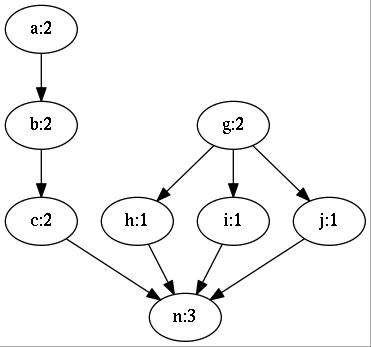
\includegraphics[width=0.9\linewidth]{fig/graph16a.jpg}
        \captionof{figure}{Graphe de test.}
      \end{center}

      \begin{titledenumerate}{Ordonnancement $P_1$.}
        \item (a:2)
        \item (b:2)
        \item (g:2)
        \item (c:2) (h:1)
        \item (i:1) (j:1)
        \item (n:3)
      \end{titledenumerate}
      \emph{Taux d'occupation de 66\%.}

      \begin{titledenumerate}{Ordonnancement $P_2$.}
        \item (g:2)
        \item (a:2) (h:1)
        \item (b:2) (i:1)
        \item (c:2) (j:1)
        \item (n:3)
      \end{titledenumerate}
      \emph{Taux d'occupation de 80\%.}
    \end{multicols}

    On suppose $N$ pair afin de simplifier l'expression. On trouve ainsi
    \[ \underbrace{N-1}_{a_{1..N-1}} + \underbrace{1}_{c} + \underbrace{1}_{a_N
    + b_1} + \underbrace{\frac{N-1}{2}}_{b_{2..N}} + \underbrace{1}_{d} =
    \frac{3N}{2} + 1 \]

    Désormais on ordonne les noeuds non plus en fonction de leur
    distance à un puits mais d'un score heuristique. Un noeud a un score égal à
    la somme des scores de ses fils plus 1. Ainsi, les puits ont un score de 1
    et ce score se propage récursivement dans le graphe.

    \newpage
  \subsection{Question 17}
    Code fourni séparément.

    \begin{multicols}{2}
      \begin{titledenumerate}{1ère heuristique}
        \item (a:2)
        \item (b:2)
        \item (c:2)
        \item (d:2)
        \item (e:2)
        \item (f:2)
        \item (o:2)
        \item (p:2)
        \item (g:2)
        \item (q:2) (u:1)
        \item (t:1) (s:1) (m:1)
        \item (l:1) (k:1) (j:1)
        \item (i:1) (h:1)
        \item (r:2)
        \item (n:3)
      \end{titledenumerate}
      \emph{Taux d'occupation de 46\%.}

      \begin{titledenumerate}{2nd heuristique}
        \item (g:2)
        \item (a:2) (u:1)
        \item (b:2) (t:1)
        \item (c:2) (s:1)
        \item (d:2) (m:1)
        \item (e:2) (l:1)
        \item (f:2) (k:1)
        \item (o:2) (j:1)
        \item (p:2) (i:1)
        \item (q:2) (h:1)
        \item (r:2)
        \item (n:3)
      \end{titledenumerate}
      \emph{Taux d'occupation de 58\%.}
    \end{multicols}
% }}}
\end{document}

% vim: set spelllang=fr:
